\cut{
\begin{itemize}
\item Compiler
  \begin{itemize}
  \item Camlp4, tcc, and fmlc (generate typedefs and prefeed defs) 
  \end{itemize}

\item Runtime system
  \begin{itemize}
  \item data structure of feed items: iData, meta data, etc
  \item implementation of feed/stream: lazy list
  \item fetching mechanism: eager fetching vs. lazy consumption, 
    http\_client library, batch fetching
  \item parse using padsML easy lib
  \item concurrency
  \item error handling
  \item discussion of selected combinators: local pairing, 
    dependent pairing (separate thread/queue)
  \end{itemize}

\item Tools library
  \begin{itemize}
  \item use of generic tool framework and feeds runtime lib
  \item use of several external ocaml libs: rrdtools, xml\_light
  \end{itemize}

\item Future work (shall we include???)
  \begin{itemize}
  \item expose meta data to the surface language
  \item a second (simplified) prefeed def with type defs only
  \end{itemize}

\item Experiments
  \begin{itemize}
  \item performance metrics: throughput, network/system latency
  \item setup (mac powerbook g4, 100Mb ethernet connection, 
    comon spec, comon nodes, random selection of nodes)
  \item two tables and graphs: throughput peaks at 
    200 nodes (chunk size), sys latency almost constant,
    system is scalable to comon (842 nodes)
  \end{itemize}
\end{itemize}
}

The implementation of the \padsd{} system comes in
three parts: the compiler, the runtime system, and the
built-in tools library. In this section, we briefly
discuss these three parts, and present some preliminary
results in the evaluation of the system performance. 
We will show that the system is robust enough and scalable to
to the size of PlanetLab type applications. 

\subsection{Compiler}
There are two parts to the \padsd{} compiler: tcc and fmlc.
tcc is the tool configuration compiler for .tc files, while fmlc is the
compiler of the feed declarations (.fml files). Both of them
compiles the source files into O'Caml programs which will
then be compiled with the run-time libraries into 
binary code. 

\begin{figure}[th]
\centering
\begin{codebox}
let simple_comon =
\{\kw{frep} = fun ff ->
 ff.\kw{all}
 \{Combinators.\kw{format} = Comon_format.Source.parse;
  \kw{print} = Comon_format.Source.print;
  \kw{format_rep} = Comon_format.Source.tyrep; 
  \kw{incremental} = false;
  \kw{header_format} = None; 
  \kw{locations} = sites;
  \kw{schedule} =
    Schedule.{\kw every} (Time.now (), 10., 
                    Schedule.default_duration, 60.);
  \kw{has_records} = Comon_format.__PML__has_records; 
  \kw{pp} = None\}\}
\end{codebox}
\caption{Code snipet of compiled simple\_comon feed}\label{fig:compiledcomon}
\end{figure}

The compilers were implemented using the Camlp4, the O'Caml
preprocessor. 
%A source program is parsed into an abstract
%syntax tree defined by the Camlp4 extended syntax, and the
%code generation is done through the quotation system. 
In the case of fmlc, the code generation is done in two steps.
In the first step, it generates type declarations for the feeds in a
lazy fashion (that is, only generate the declaration if the
feed is used in the rest of the description).
In the second step, it generates the feed representation,
also known as the ``prefeed''. Schedules which are
definite times such as ``2008/09/30:12:00:00'' or ``5 mins'' are
converted to floating point number of seconds at compile time
to make the code more efficient.
All O'Caml expressions embeded in the fml file are
included without change in the compiled code. 
Figure \ref{fig:compiledcomon} shows the compiled code for
the simple CoMon feed in Figure \ref{fig:simplecomon}.

\subsection{Runtime System}
A feed in \padsd{} is implemented as a lazy list of feed
items (known as idata). This means the feed 
is actually a function {\tt next}. It is evaluated 
only when the user program attempts to take an
item from the feed. The function {\tt next} returns an
item plus a new {\tt next} function which represents
the tail of the feed.

An idata is a pair of a data item of polymorphic type 'a and 
a meta data structure that corresponds 'a. 
%The type of a feed is also the type of its data item. 
%The type of a base feed has an option type. 
The meta data is a tree structure in which
each node is tagged with a meta header. 
The tree structure (also known as the meta body) resembles 
the structure of the data item, i.e.  if the data item is a pair, 
then the meta body is also a pair of meta data. Each leaf
of the meta body corresponds to a base feed. Meta information
such as the scheduled time, arrival time, location and 
errors is stored in the leaves. The header records the summary 
of meta information within the subtree. 

The \padsd{} runtime system is a multi-threaded concurrent
system. Each base feed is created and maintained by a separate 
worker thread, and a master thread drives the combination of 
base feeds into compound feeds. Each worker thread and the 
master thread communicate through a concurrent queue.
Basically, each worker thread fetches data from the specified
location , parses the data into internal representation 
(known as the {\em rep})
using the \padsml parser, or synthesize data by calling a function.
And then it generates the idata from the rep and the meta data,
and pushes the idata into the concurrent queue.
The master thread pops the idata from the queue {\em on demand}, that is,
when the data is requested by the user program. In other words,
the worker thread is {\em eager}, while the master thread is {\em lazy}.
The concurrency control is implemented by the O'Caml threads
library using standard mutex and condition variables.

The fetching engine is implemented using
the Ocamlnet 2 library which is capable of concurrent fetches. 
Given a list of locations to fetch from at any one time, 
we convert the list into batches and fetch up to 200 locations
per batch. The choice of 200 is a trade-off between maximizing
the throughput and avoiding overwhelming the operating system
with too many open sockets. If the system fails to fetch an
item due to network or system error, an idata is still created
with the appropriate error code written in the meta data and
{\em None} set as the data value. Some of error codes include:
{\small \begin{verbatim}
1: Misc HTTP error
2: Late arrival
3: Ssh host required
4: Remote command required for ssh
5: Bad message
\end{verbatim}}
The \padsd{} system does not 
automatically filter out erroneous items because errors often 
provides very important information to users who monitors 
distributed systems. Users could optional choose to filter
out bad feed items using the Feed library functions.

Compound feeds are created within the generic tool framework by
combining base feeds using various combinator functions.
These functions takes idatas from two feeds and creates a new idata often
by comparing the timestamps in the two idatas. While this is done
lazily in most of the combinators, it is not the case for
dependent pairs. This is because the dependent feed needs to be
created {\em eagerly} when each item from the {\em depending}
feed arrives. Therefore we add another layer of ``pseudo-fetching"
for the dependent feed. Here a separate thread is created for each
dependent feed, which actively takes data from the depending
feed, creates dependent items, and push to another concurrent
queue of its own.  
 
\subsection{Tools Library}
Most of the built-in tools were implemented under the
generic tools framework with the prefeed as the traversal
function. The feed selector relies on a selector tool
for \padsml{} which selects into a \padsml{} type following
a certain path. The feed2rrd tool requires the installation
of the rrdtool package which is a round-robin database. 
The feed2rss tool uses the XML-Light package which
is a minimum XML parser and printer for O'Caml.
The system also provides an Feed interface to a number of
useful runtime functions such as map and fold for advanced
users to program against the feeds.

\begin{table*}[th]
\begin{center}
\begin{tabular}{|l|r|r|r|r|r|r|r|r|r|r|r|r|}\hline
Num of nodes&	50&	100&	150&	200&	250&	300&	350&	400&	450&	500&	550&	600 \\ \hline\hline
Net latency per node (secs)&	9&	4&	4&	4&	8.6&	5.3&	19.1&	19.5&	14.4&	7.8&	12&	13.3 \\ \hline
Sys latency per node (secs)&	0&	0&	0&	0.3&	0.2&	0.4&	0.3&	0.1&	0.3&	0.4&	0.2&	0.7 \\ \hline
%Total Latency (secs)&	9&	4.04&	4&	4.3&	8.8&	5.8&	19.4&	19.6&	14.7&	8.2&	12.3&	14 \\ \hline
Total fetch time (secs)&	9&	5&	4&	5&	23&	9&	22&	23&	26&	14&	27&	28 \\ \hline	
Throughput (items/sec)&	5.6&	20&	37.5&	40&	10.9&	33.3&	15.9&	17.4&	17.3&	35.7&	20.4&	21.4 \\ \hline
\end{tabular}
\end{center}
\caption{Performance of CoMon without archiving}
\label{tab:comon-noarch}
\end{table*}


\begin{table*}
\begin{center}
\begin{tabular}{|l|r|r|r|r|r|r|r|r|r|r|r|r|}\hline
Num of nodes&	50&	100&	150&	200&	250&	300&	350&	400&	450&	500&	550&	600 \\ \hline\hline
Net latency per node (secs)&	16&	4&	4&	4&	18.9&	6&	20.6&	22&	8.4&	13&	21.8&	21.3 \\ \hline
Sys latency per node (secs)&	0.8&	1.28&	1.4&	1.8&	1.9&	1.5&	1.6&	1.3&	1.9&	1.7&	1.7&	2.2 \\ \hline
%Total Latency (secs)&	16.8&	5.28&	5.4&	5.8&	20.8&	7.5&	22.2&	23.3&	10.3&	14.7&	23.56&	23.5 \\ \hline
Total fetch time (secs)&	17&	6&	7&	7&	27&	12&	27&	30&	19&	33&	43&	43 \\ \hline
Throughput (items/sec)&	2.9&	16.7&	21.4&	28.6&	9.3&	25&	13&	13.3&	23.7&	15.2&	12.8&	14 \\ \hline
\end{tabular}
\end{center}
\caption{Performance of CoMon with archiving}
\label{tab:comon-arch}
\end{table*}

\subsection{Preliminary Experiments} \label{sec:experiments}
As a preliminary performance evaluation, 
we measure the average network latency
to fetch a data item, the average system latency 
to produce a data item
and the total throughput of the system using the CoMon feed
description in Figure \ref{fig:feedcomon}. 
The throughput measures the average
number of locations fetched per second. We picked
the comon example because it is a real life
application that involves fetching from large number of 
nodes (up to 842 nodes at the time of writing)
at the same time, which can be viewed as a stress test. 

All the experiments were conducted on a Mac Powerbook G4 computer
with a 1.67GHz CPU and 2GB memory running Mac OS X 10.4. It is
connected to the internet through a 100Mb/s ethernet. 
We randomly select 50, 100, and up to 600 nodes from the 
real CoMon node list, 
\footnote{List taken from http://www.cs.princeton.edu/~vivek/node\_list\_all. 
Not all nodes are up at the same time.}
and use these smaller node lists as a total of 12 test cases. 

Tables \ref{tab:comon-noarch} and \ref{tab:comon-arch}
shows the results from two different scenarios:
one in which the user program simply creates the comon feed without applying
any tools on it, and one in which the comon feed is created
and archived. In both scenarios, the system was
able to fetch from up to 600 nodes within one minute, which is
significantly shorter than the 5-minute turnaround time in the real
CoMon system.

\begin{figure}[th]
\begin{center}
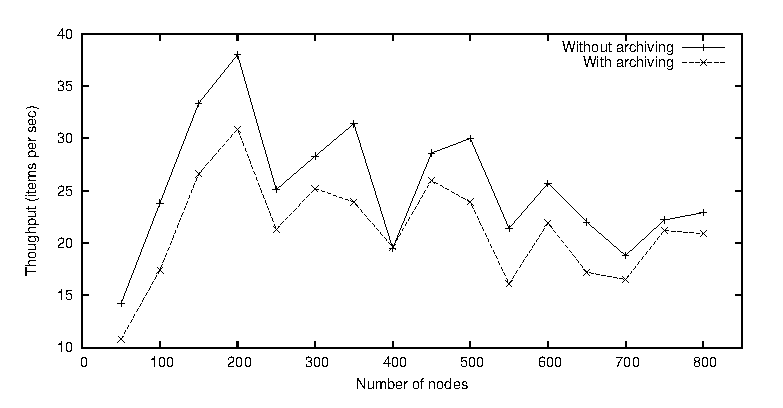
\epsfig{file=throughput.eps, width=\columnwidth}
\caption{Average throughput}
\label{fig:throughput}
\end{center}
\end{figure}

\begin{figure}[th]
\begin{center}
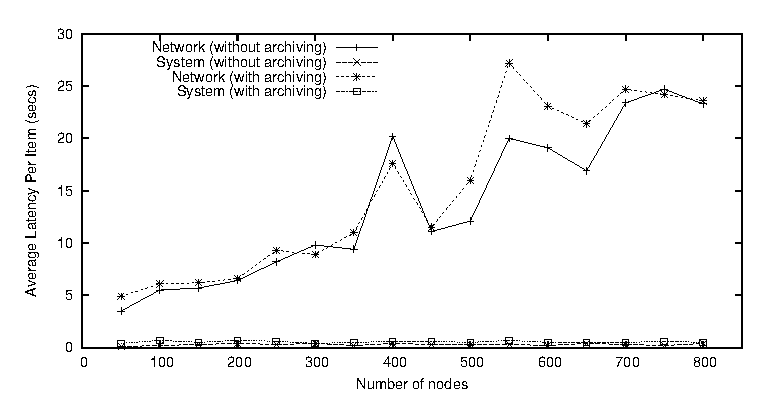
\epsfig{file=latency.eps, width=\columnwidth}
\caption{Average latencies per node}
\label{fig:latency}
\end{center}
\end{figure}

We plot the average throughput in Figure \ref{fig:throughput}
and the system and network latencies in Figure \ref{fig:latency}. 
As expected, both the thoughput and latency suffer a little with 
archiving taking place. The throughput peaks when fetching from
200 nodes because 200 is the size of the fetching batch and
at 200 nodes, the concurrent fetching engine is maximally utilized.
The experiment for 450 nodes exhibits an anomaly as the archived
experiment takes less time than the un-archived experiment.
This is probably due to sudden delays in some of the nodes when the
no-archiving experiment is run. One obvious take-away from
Figure \ref{fig:latency} is that while the network latency may
vary greatly depending on the network condition, the system latency
stays almost constant at relatively low levels. This shows that
the \padsd{} system runtime adds little overhead to the 
inevitable network cost, which means the system could scale to
large applications. 

